\begin{bx1}
  \begin{wrapstuff}[type=figure,r,lines=7,width=0.23\linewidth]
    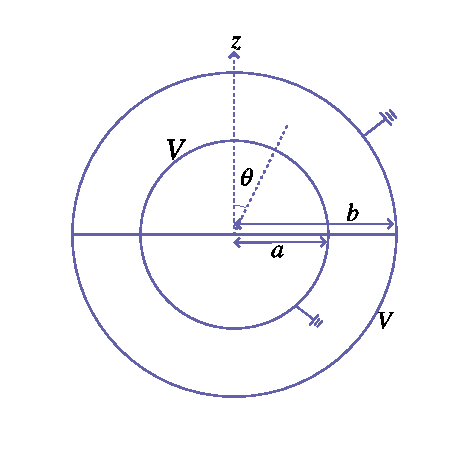
\includegraphics[width=\linewidth]{fig/Jackson3-1.pdf}%  
  \end{wrapstuff}
  共通中心を持つ2つの球(それぞれの半径は$a, b$で与えられ,$b>a$を満たす)があり,それぞれは
  共通の水平板によって2つの半球に分割されている.内部の球の上側と外側の球の下側のポテンシ
  ャルは$V$に固定され,その他の半球のポテンシャルはゼロに固定されている.

  このとき,$a \leq r \leq b$の領域におけるポテンシャルをLegendre多項式による展開として
  決定せよ.このとき,少なくとも$l = 4$の項までを含めよ.ここで得られた結果と,
  よく知られた結果である$b \to \infty$や$a \to 0$の場合と比較せよ.
\end{bx1}
半径$a, b$の球の間の領域のポテンシャルを考える.Legendre多項式による展開
\begin{gather}%
  \Phi(r, \theta) = \sum_{l=0}^\infty \ab(A_l r^l + B_l r^{-(l+1)}) P_l (\cos\theta)
\end{gather}
を以下の境界条件で考える:
\begin{gather}%  
  \label{eq:prob3-1_bc1}
  \Phi(a,\theta) =
  \begin{dcases}%
    V \qqtext{if} 0 \leq \theta \leq \frac{\pi}{2}\\
    0 \qqtext{if} \frac{\pi}{2} \leq \theta \leq \pi
  \end{dcases},\\
  \label{eq:prob3-1_bc2}
  \Phi(b,\theta) =
  \begin{dcases}%
    0 \qqtext{if} 0 \leq \theta \leq \frac{\pi}{2}\\
    V \qqtext{if} \frac{\pi}{2} \leq \theta \leq \pi
  \end{dcases}% 
\end{gather}%
\eqref{eq:prob3-1_bc1}について,$P_{l'}(\cos\theta)\dl{(\cos\theta)}$をかけて$\theta\in[0,\pi]$
で積分をすると,
\begin{gather}%
  \int_{\cos\theta=1}^{\cos\theta=-1} \sum_{l=0}^\infty\ab(A_la^l + B_la^{-(l+1)})
  P_l(\cos\theta) P_{l'}(\cos\theta) \dl{(\cos\theta)} 
  =  V \int_{\cos\theta=1}^{\cos\theta=0} P_{l'}(\cos\theta) \dl{(\cos\theta)}
\end{gather}
である.左辺の積分変数を$x$で書くと,
\begin{gather}%
  \text{(L.H.S.)} = \int_{1}^{-1} \sum_{l=0}^\infty\ab(A_l a^l + B_l a^{-(l+1)})
  P_l(x) P_{l'}(x) \dl{x}
\end{gather}
であり,Legendre多項式に関する直交関係\eqref{eq:legendre_orthogonal}より,($l,l'$を入れ替えて)
\begin{gather}%
  \label{eq:prob3-1_a}
  A_l a^l + B_l a^{-(l+1)} = \frac{V(2l+1)}{2} \int_0^1 \dl{x} P_l(x)
\end{gather}%
を得る.
同様に考えて,\eqref{eq:prob3-1_bc2}について,
\begin{gather}%
  \label{eq:prob3-1_b}
  A_l b^l + B_l b^{-(l+1)} =(-1)^l \frac{V(2l+1)}{2} \int_0^{1} \dl{x} P_l(x)
\end{gather}%
が成り立つ.
ただし,$P_l(-x) = (-1)^l P_l(x)$に注意せよ.

式\eqref{eq:prob3-1_a}と\eqref{eq:prob3-1_b}より,係数$A_l, B_l$を計算することができて,
\begin{gather}%
  A_l = \frac{(-1)^lb^{l+1}-a^{l+1}}{b^{2l+1}-a^{2l+1}}
  \frac{V(2l+1)}{2} \int_0^1 \dl{x} P_l(x),\\
  B_l = \frac{b^l-(-1)^la^l}{b^{2l+1}-a^{2l+1}}a^{l+1}b^{l+1}
  \frac{V(2l+1)}{2}\int_0^1 \dl{x} P_l(x)
\end{gather}%
がわかる.
したがって,ポテンシャルの正確な形は
\begin{gather}
  \Phi(r,\theta) =
  V \sum_{l=0}^\infty \ab(
  \frac{(-1)^lb^{l+1}-a^{l+1}}{b^{2l+1}-a^{2l+1}} r^l +
  \frac{b^l-(-1)^la^l}{b^{2l+1}-a^{2l+1}}a^{l+1}b^{l+1} r^{-(l+1)}
  )
  \times\frac{2l+1}{2}\ab(\int_0^1 \dl{x} P_l(x))
  P_l(\cos\theta)
\end{gather}

である.
具体的に$l = 4$の項までを書き下せば,
\begin{gather}
  \Phi(r,\theta) = V \left[
    \frac{1}{2} + \frac{3}{4}\frac{-(a^2+b^2)r+a^2b^2(a+b)r^{-2}}{b^3-a^3} P_1(\cos\theta)\right.
    \left.
    -\frac{7}{16}\frac{-(a^4+b^4)r^3 + a^4b^4(a^3+b^3)r^{-4}}{b^7-a^7}P_3(\cos\theta) +\cdots
    \right]
\end{gather}
となる.

$b \to \infty$の極限では$a/b \to 0, r/b\to 0$として,
\begin{align}%
  \Phi(r,\theta) 
  &= V
  \sum_{l=0}^\infty \frac{2l+1}{2}\ab(\frac{a}{r})^{l+1}
  \ab(\int_0^1\dl{x} P_l(x)) P_l(\cos\theta)\notag\\
  &= V\ab[
    \frac{1}{2} + \sum_{k=0}^\infty \frac{(-1)^k(4k+3)(2k-1)!!}{2^{k+2}(k+1)!} 
    \ab(\frac ar)^{2k+2} P_{2k+1}(\cos\theta)
  ]\\
  &= V\ab[
    \frac{1}{2} + \frac{3}{4}\ab(\frac{a}{r})^2 P_1(\cos\theta) -
    \frac{7}{16}\ab(\frac{a}{r})^4 P_3(\cos\theta) + \cdots
  ]
\end{align}%
である.
ただし,ここでは$(-1)!! = 1$と約束する.
これは半径$a$の導体球について,
北半球のポテンシャルが$V$,南半球が接地されており,さらに
無限遠でのポテンシャルの境界条件が$V/2$となる系において,導体球の外部領域に作る
ポテンシャルに等しいことがわかる.

$a \to 0$の極限では
\begin{align}%
  \Phi(r,\theta) &= V \sum_{l=0}^\infty (-1)^l \frac{2l+1}{2} \ab(\frac rb)^{l} 
  \ab(\int_0^1\dl{x} P_l(x)) P_l(\cos\theta)\notag\\
  &= V\ab[\frac 12 + \sum_{k=0}^\infty \frac{(-1)^{k+1}(4k+3)(2k-1)!!}{2^{k+2}(k+1)!}
  \ab(\frac rb)^{2k+1} P_{2k+1} (\cos\theta)]\\
  &= V\ab[\frac 12 - \frac 34 \ab(\frac rb) P_1(\cos\theta) +
  \frac{7}{16}\ab(\frac rb)^3P_3(\cos\theta)]
\end{align}%
である.
これは,半径$b$の導体球について,
北半球が接地されていて,南半球のポテンシャルが$V$となるような系における,
球内部のポテンシャルに等しいことがわかる.

それぞれの場合について,ポテンシャルを描く
と図\ref{fig:3-1_lima},\ref{fig:3-1_limb},\ref{fig:3-1_all}のようになる\footnote{
  描画のときに使用したコードは\texttt{.ipynb}形式で保存してある.
}.
\begin{figure}[htbp]%  
  \centering%  
  \begin{minipage}{0.30\linewidth}
    \centering
    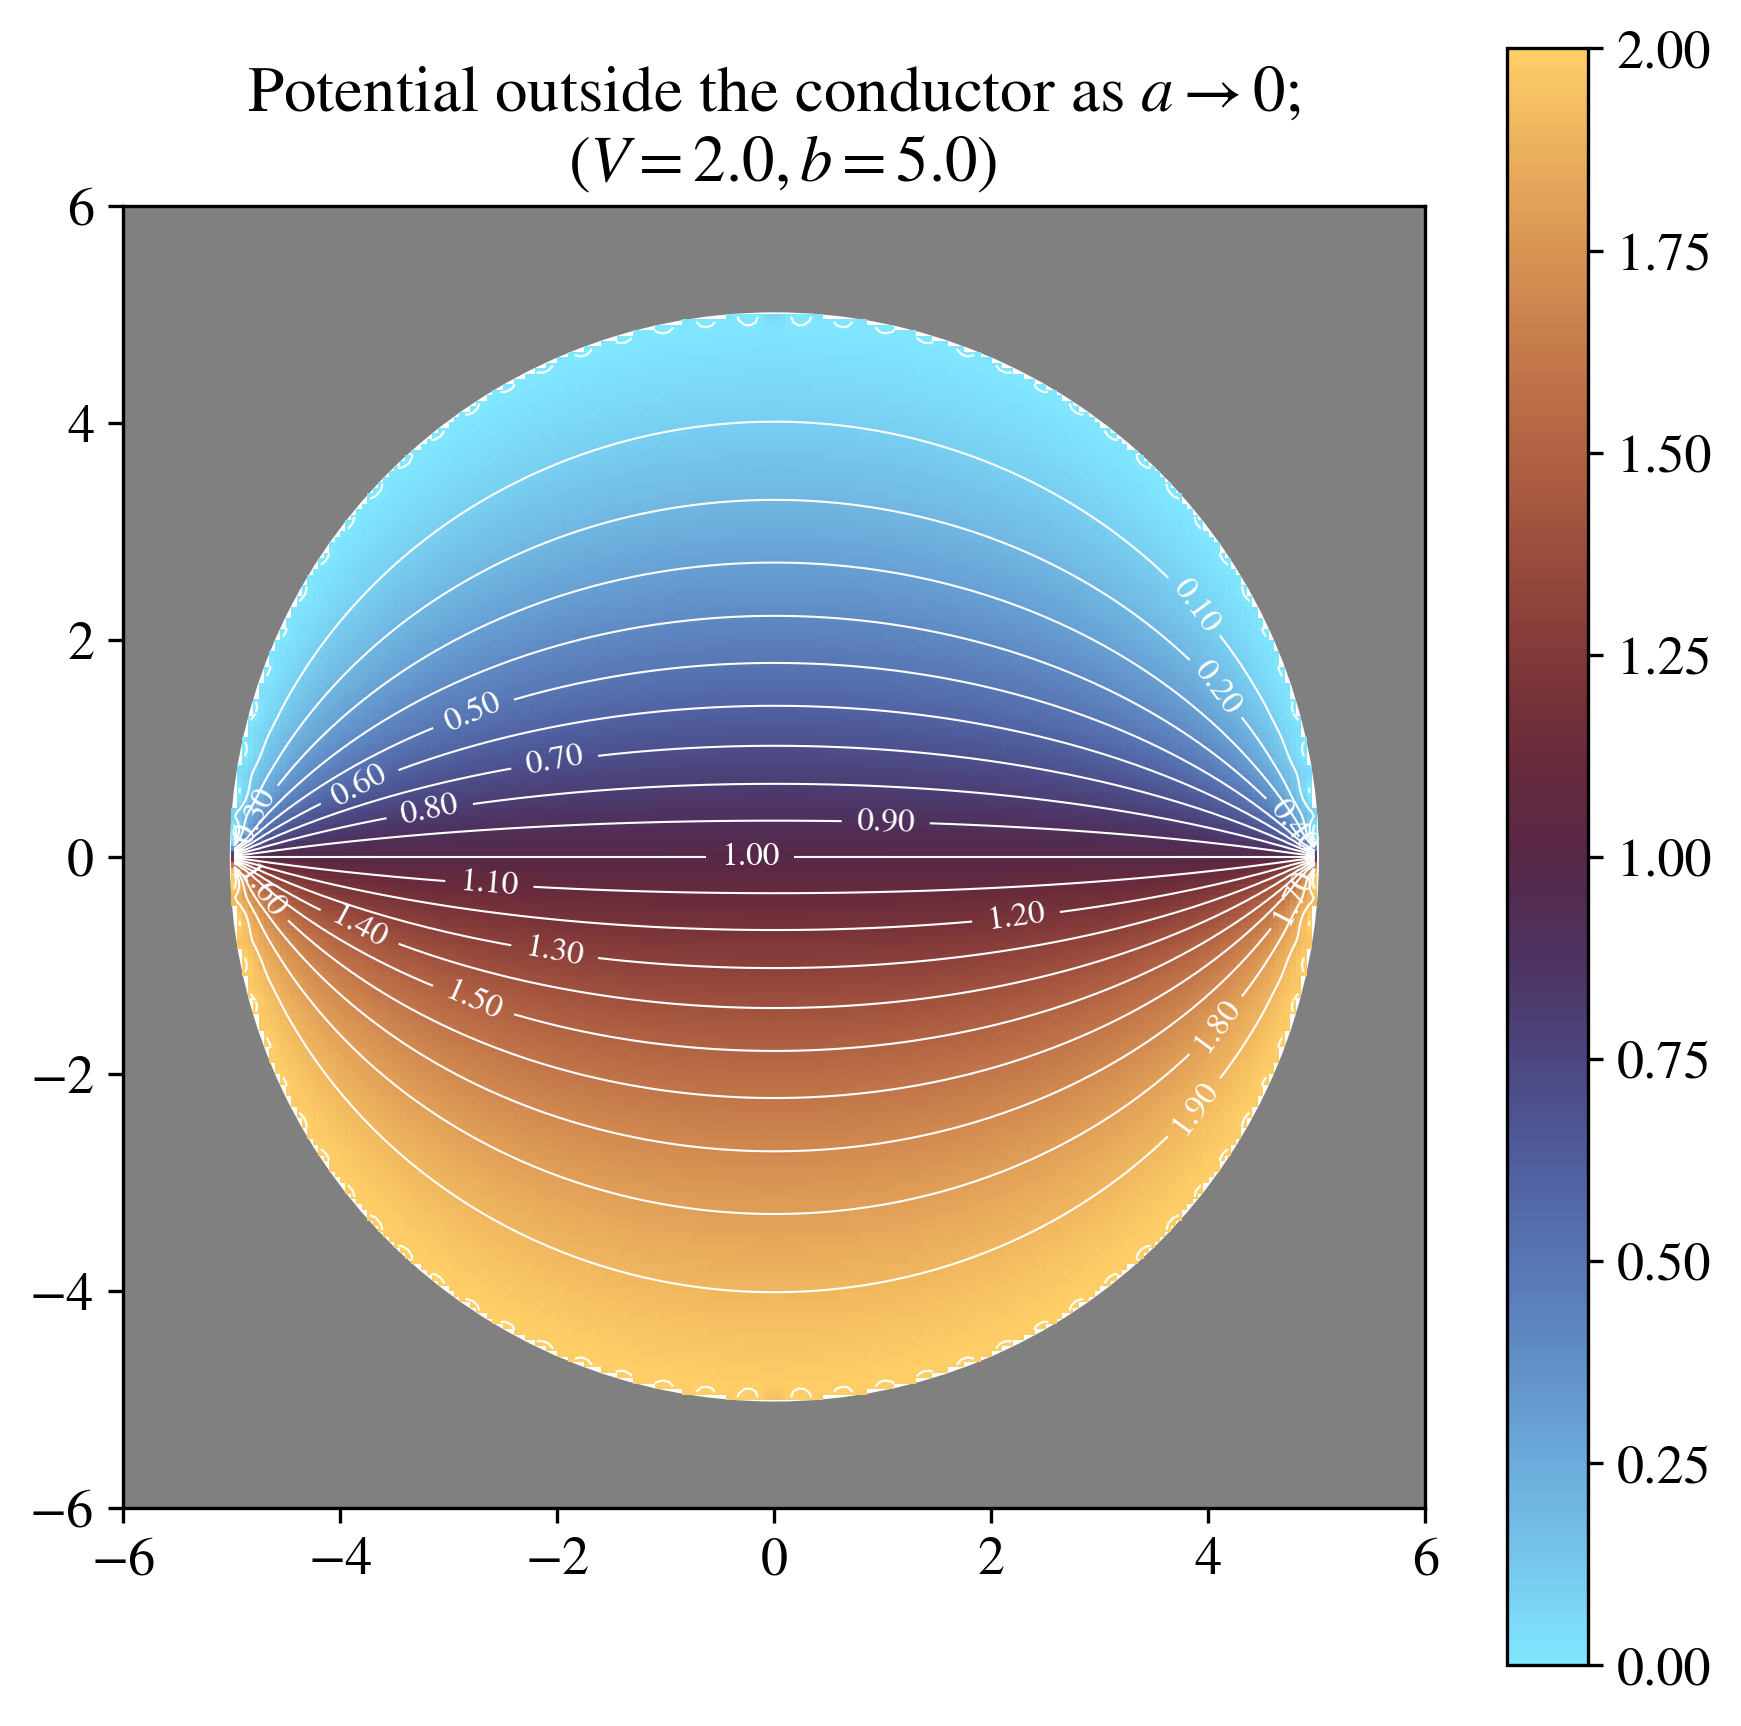
\includegraphics[width=\linewidth]{py/3-1_lima.png}%  
    \caption{$a \to 0$としたときのポテンシャル}%  
    \label{fig:3-1_lima}%  
  \end{minipage}
  \begin{minipage}{0.30\linewidth}
    \centering
    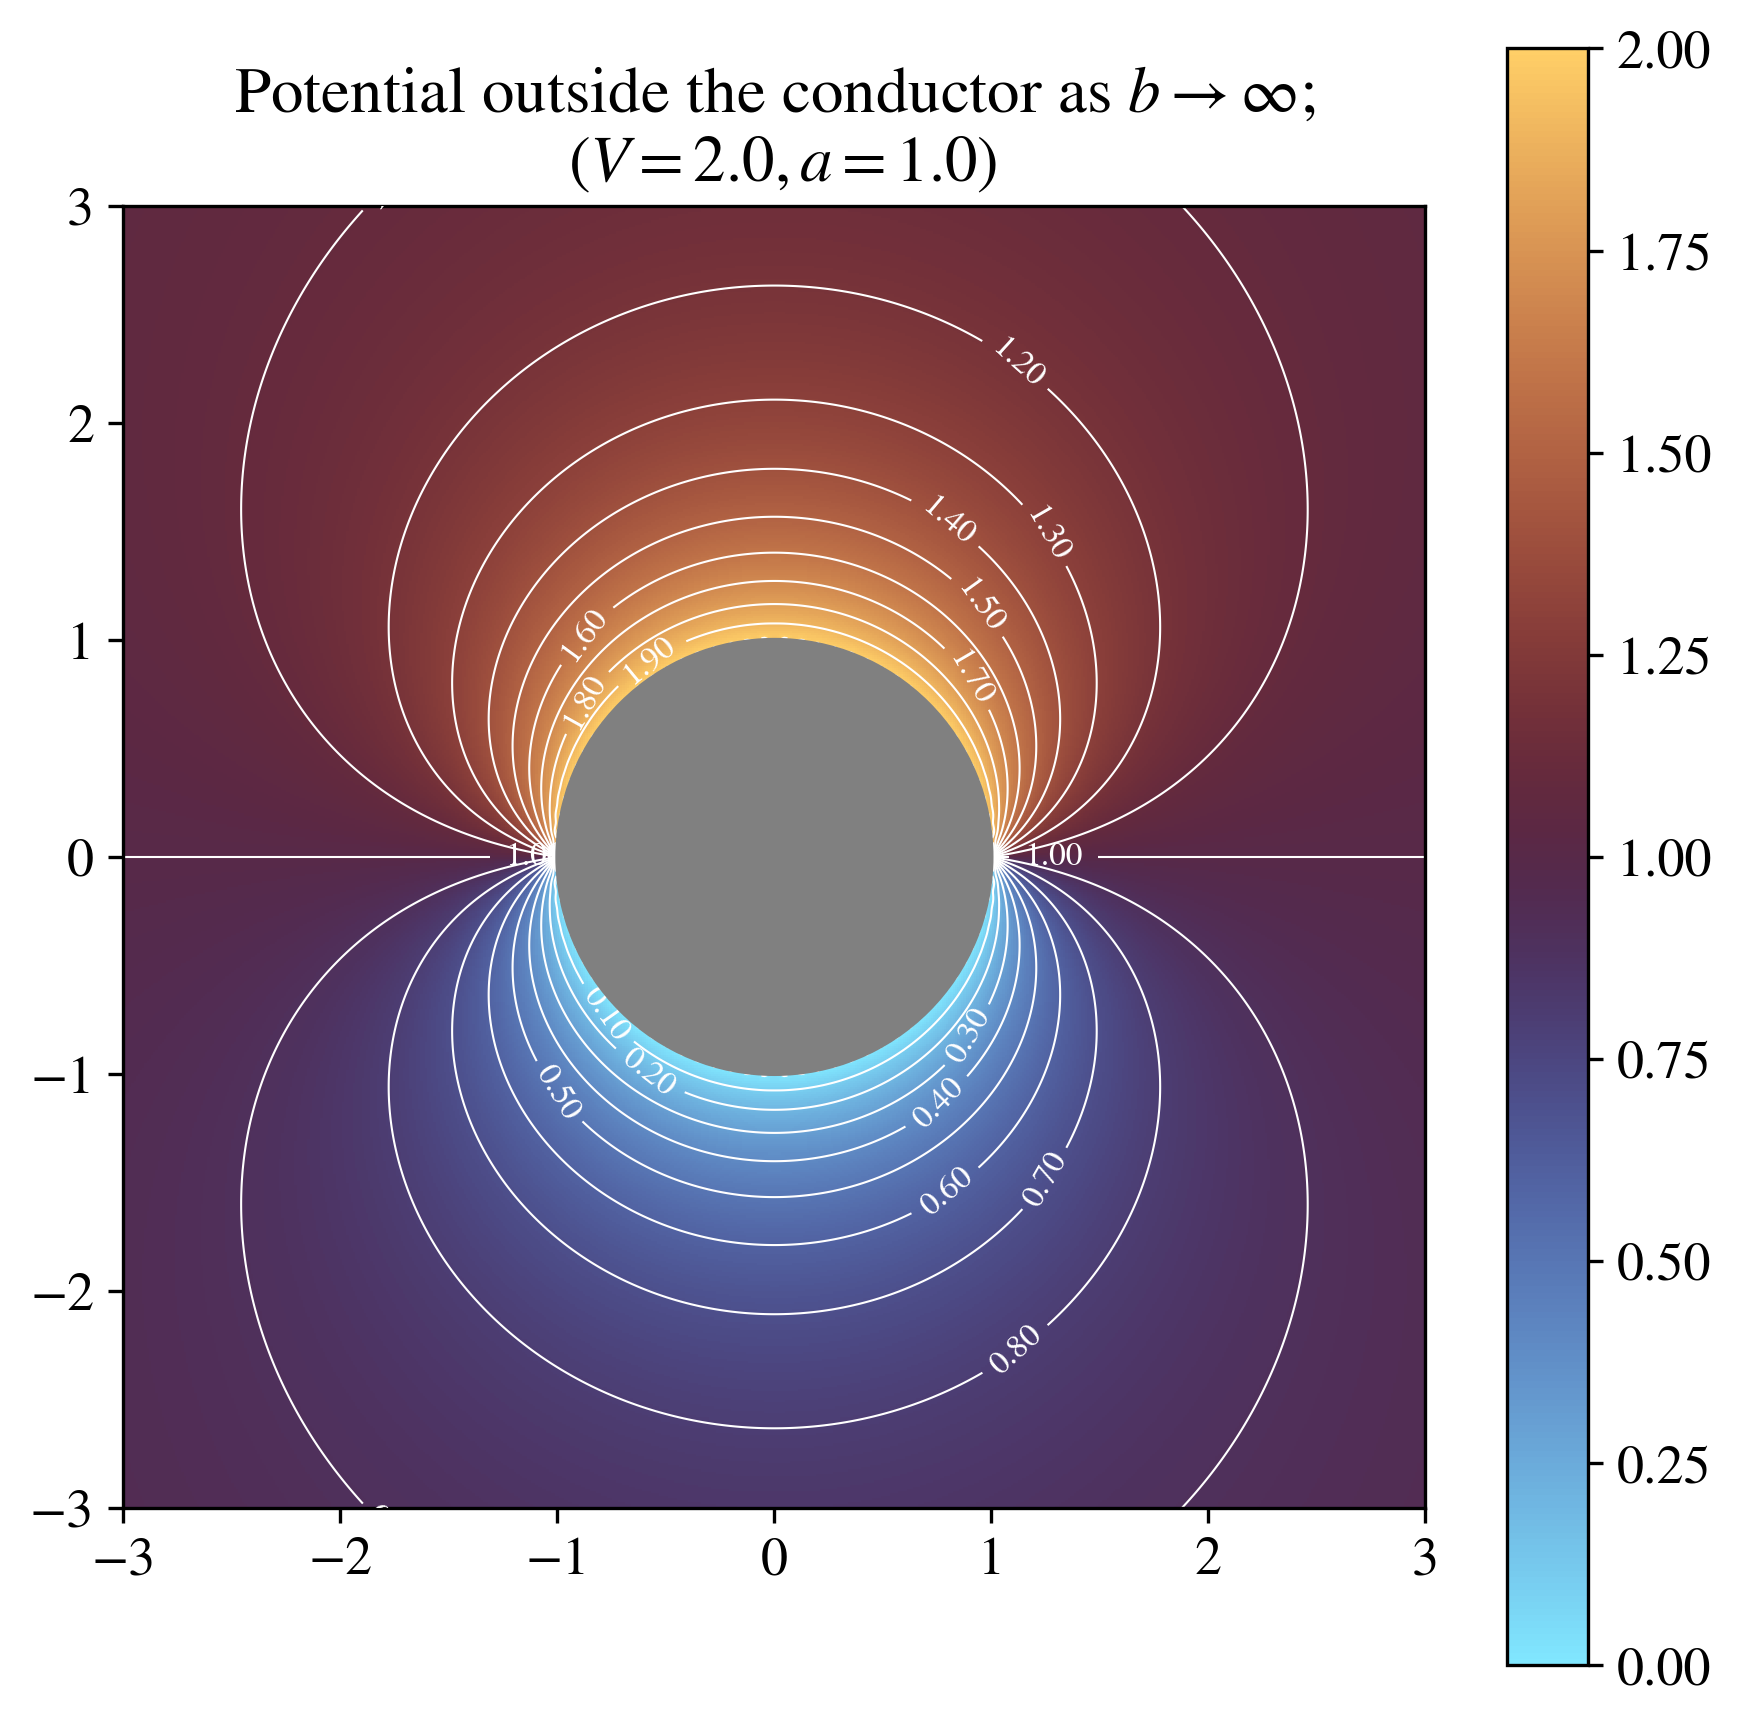
\includegraphics[width=\linewidth]{py/3-1_limb.png}%  
    \caption{$b\to\infty$としたときのポテンシャル}%  
    \label{fig:3-1_limb}%  
  \end{minipage}
  \begin{minipage}{0.30\linewidth}
    \centering
    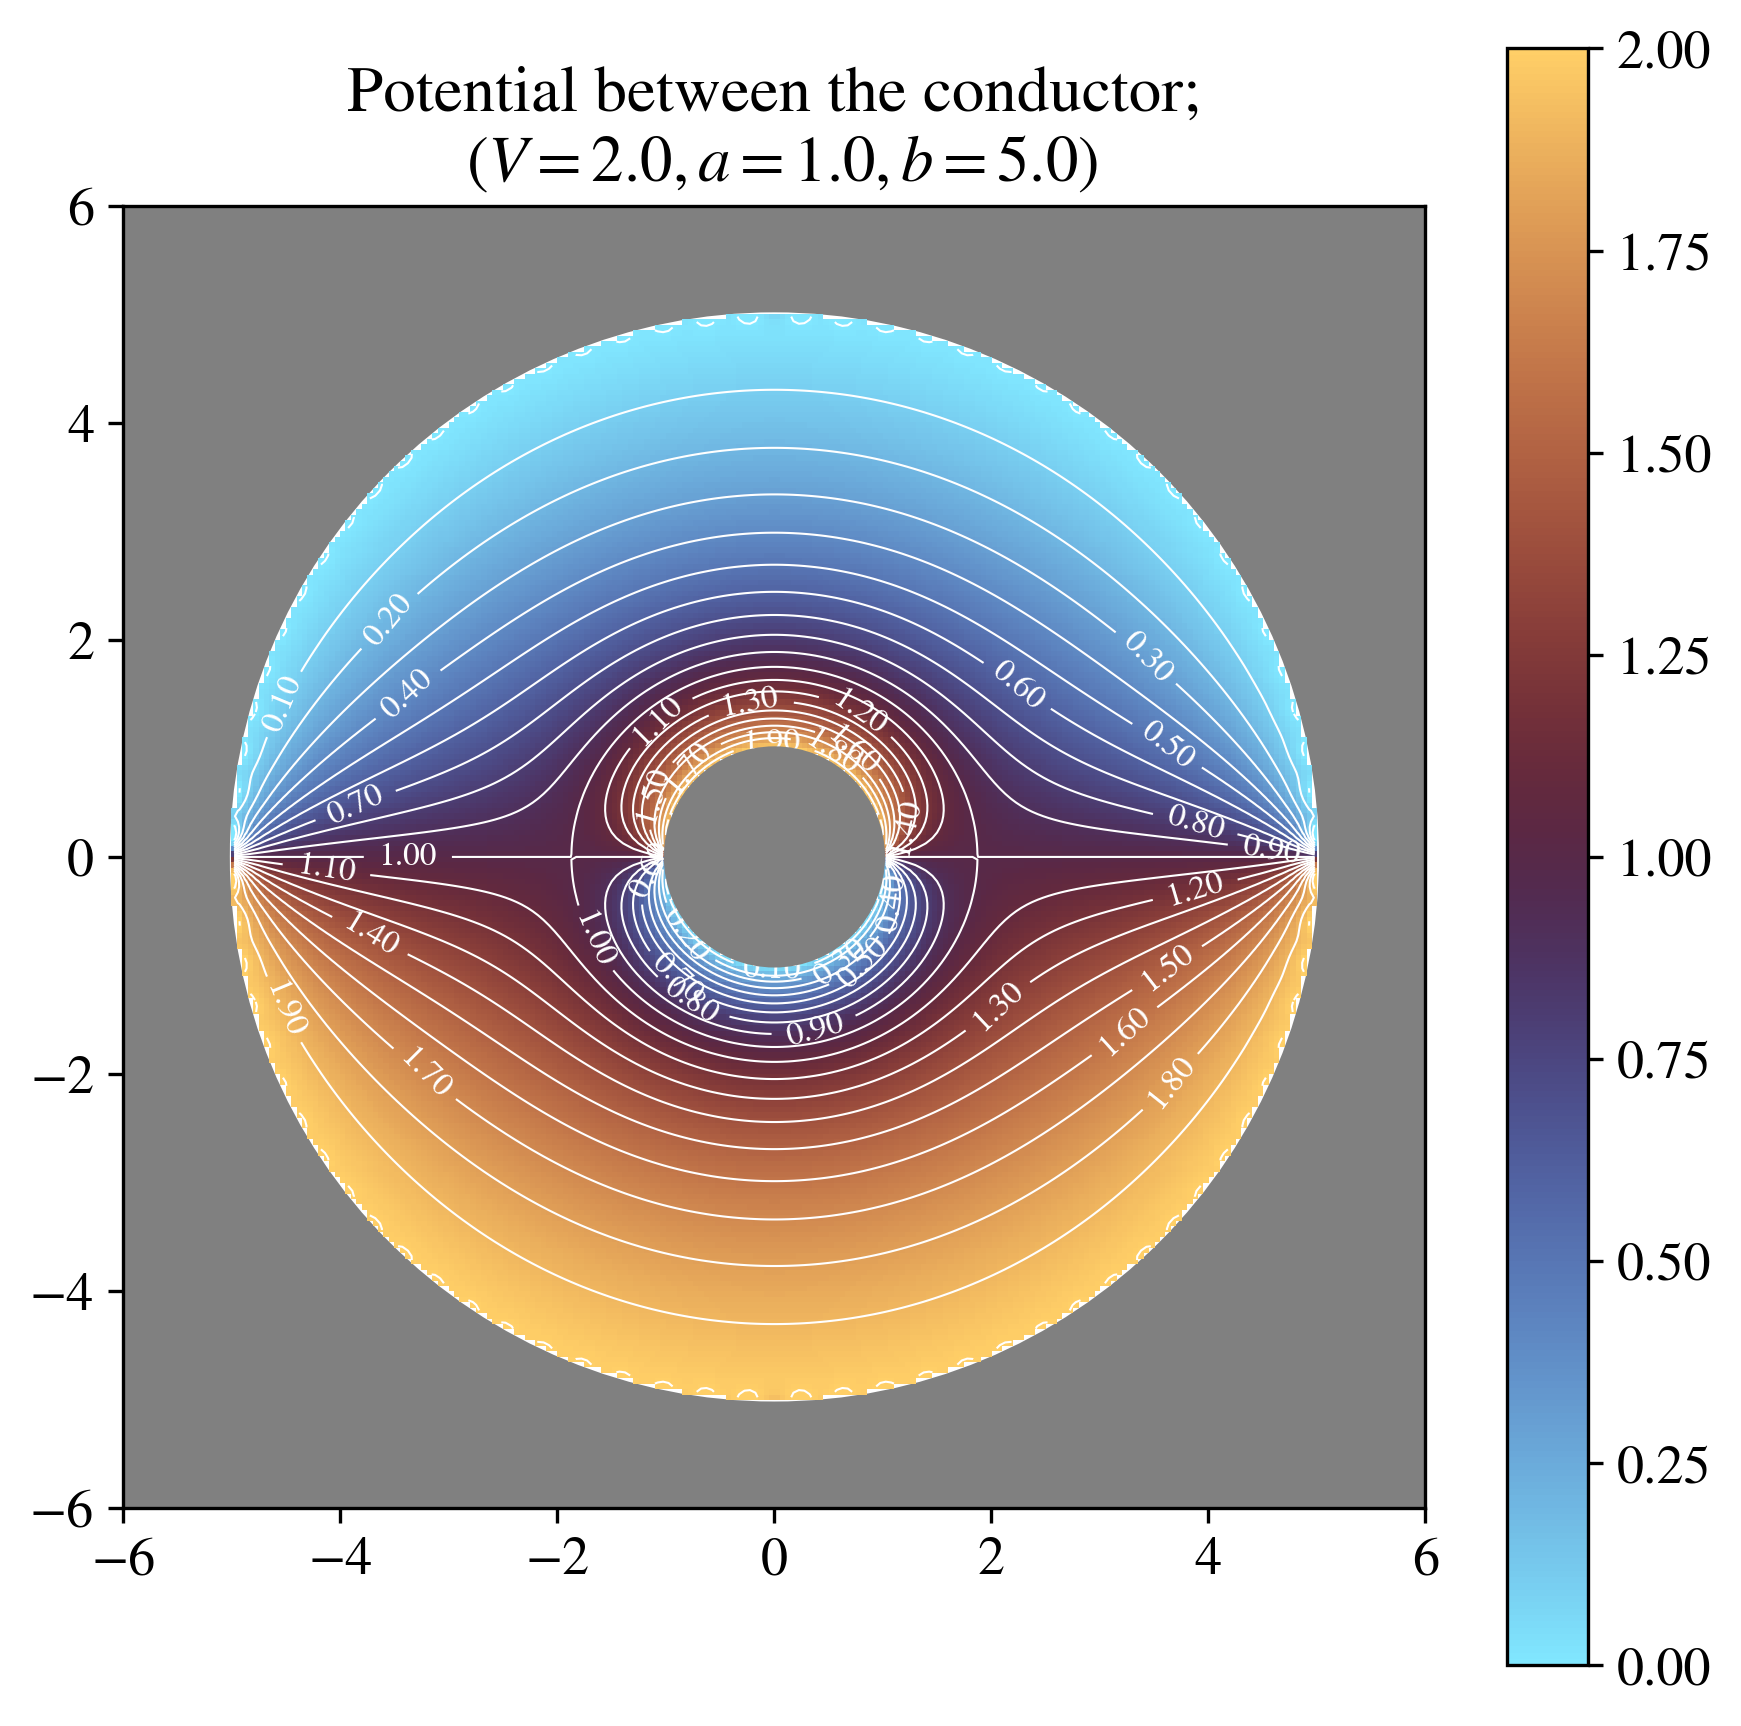
\includegraphics[width=\linewidth]{py/3-1_all.png}
    \caption{一般の場合についてのポテンシャル}
    \label{fig:3-1_all}
  \end{minipage}
\end{figure}%

\clearpage
